% !TeX root = ../main.tex

\section{CI/CD}
    \begin{frame}{Mobile Application Development Lifecycle}
        Per poter automatizzare un processo è necessario prima comprendere da quali task è composto e le relazioni tra di essi:
        \begin{columns}[onlytextwidth]
            \begin{column}{0.4\textwidth}
                \begin{itemize}
                    \item Pianificazione
                    \item Progettazione
                    \item Sviluppo
                    \item Stabilizzazione
                    \item Release
                    \item Monitoring
                \end{itemize}
            \end{column}
            \begin{column}{0.6\textwidth}
                \begin{figure}[H]
                    \centering
                    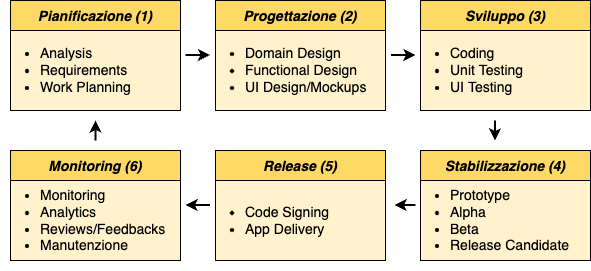
\includegraphics[width=1\textwidth]{img/tesi-2-Page-9.drawio.png}
                \end{figure}    
            \end{column}
       \end{columns}
    \end{frame}


%    \begin{frame}{Pipeline Obiettivo}
%        \begin{itemize}
%            \item I task del processo a cui sono applicate le tecniche di Continuous Integration e Continuous Delivery sono \textit{Sviluppo}, \textit{Stabilizzazione} e \textit{Release}.
%            \item Non esiste il concetto di deployment automatizzato nel mondo delle applicazioni mobile: l'applicazione viene rilasciata tramite pubblicazione sull'apposito store e l'utente effettua in un secondo momento l'installazione sul proprio dispositivo.
%            \item Dato il vincolo tecnologico del framework KMM per lo sviluppo della applicazione, la pipeline è stata progettata utilizzando come caso d'uso l'applicazione base generata con il plugin Gradle KMM.
%        \end{itemize}
%    \end{frame}

    \begin{frame}{Branching Model}
        \begin{columns}[onlytextwidth]
            \begin{column}{0.5\textwidth}
                \begin{itemize}
                    \item Fondamentale per l'efficacia del processo progettato
                    \item Basato su GitFlow
                    \item 3 branch principali:
                    \begin{itemize}
                        \item \textit{dev} (alpha)
                        \item \textit{test} (beta)
                        \item \textit{main} (prod)
                    \end{itemize}
                \end{itemize}
            \end{column}
            \begin{column}{0.5\textwidth}
                \begin{figure}[H]
                    \centering
                    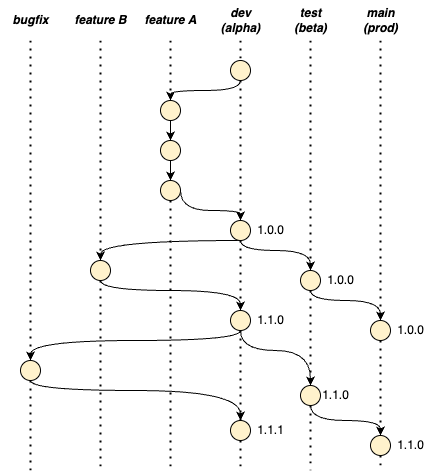
\includegraphics[width=1\textwidth]{img/tesi-13-branching.drawio.png}
                \end{figure}
            \end{column}
        \end{columns}
    \end{frame}
    
    \begin{frame}{Pipeline Obiettivo}
        \begin{figure}[H]
            \centering
            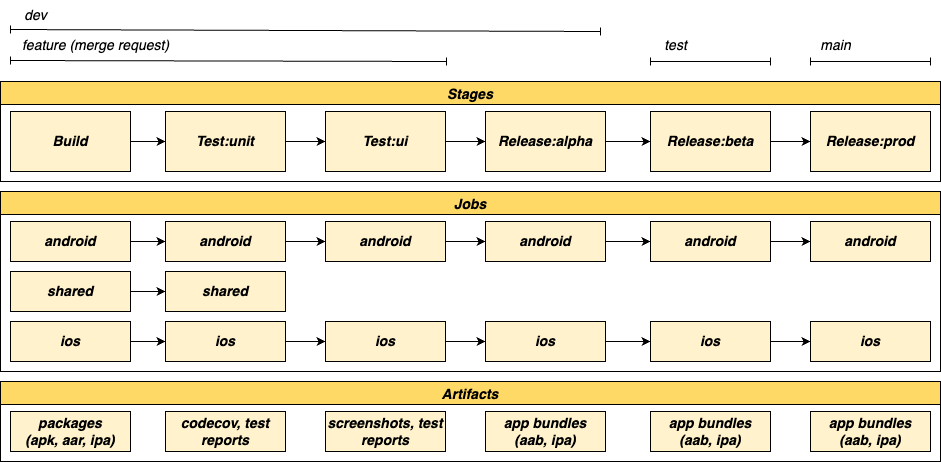
\includegraphics[width=1\textwidth]{img/tesi-2-Page-12.drawio.png}
        \end{figure}  
    \end{frame}

    \begin{frame}{Continuous Integration}

    \end{frame}

    \begin{frame}{Continuous Delivery}

    \end{frame}

    \begin{frame}{Continuous Inspection}

    \end{frame}